\tikzset{
  fncSty/.style={font=\footnotesize, align=center},
  meshSty/.style={font=\footnotesize, align=center, draw=darkgray, rounded corners=0.5ex},
  arrowSty/.style={->, >=latex, draw=darkgray, thick},
  arrowLabelSty/.style={font=\scriptsize, align=center},
}
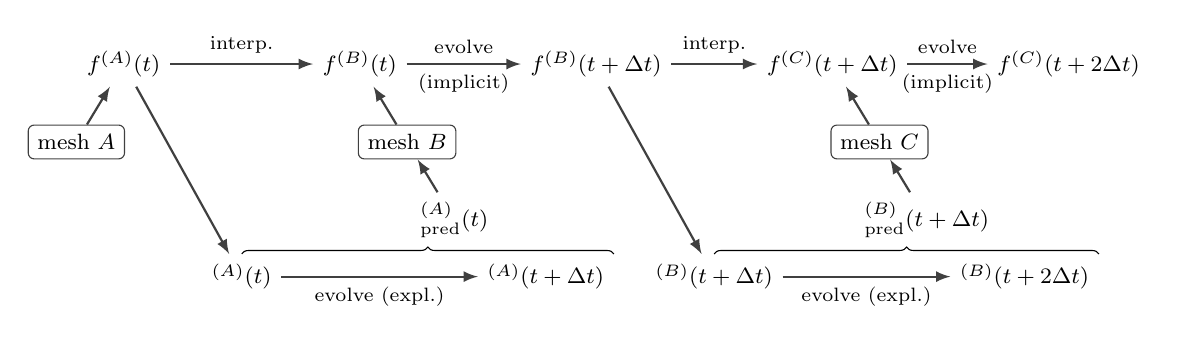
\begin{tikzpicture}
  \def\dh{3.0}
  \def\dv{0.9}

  \node[fncSty]   (fA1) at (-0.5*\dh,-0.0*\dv) {$f^{(A)}(t)$};
  \node[meshSty]  (mA)  at (-0.7*\dh,-1.1*\dv) {mesh $A$};
  \draw[arrowSty] (mA) -- (fA1);

  \node[fncSty]             (iA1) at (0*\dh,-3*\dv) {$\indfn^{(A)}(t)$};
  \node[fncSty,anchor=west] (iA2) at (1*\dh,-3*\dv) {$\indfn^{(A)}(t + \Delta t)$};
  \draw[arrowSty] (iA1) -- node[arrowLabelSty,below]{evolve (expl.)} (iA2);
  \draw[arrowSty] (fA1) -- (iA1);

  \draw[decoration={brace},decorate] (iA1.north) -- (iA2.north east);
  \node[fncSty]   (pA2) at (0.9*\dh,-2.2*\dv) {$\indfn^{(A)}_\mathrm{pred}(t)$};
  \node[meshSty]  (mB)  at (0.7*\dh,-1.1*\dv) {mesh $B$};
  \draw[arrowSty] (pA2) -- (mB);

  \node[fncSty]   (fB0) at (0.5*\dh,-0*\dv) {$f^{(B)}(t)$};
  \draw[arrowSty] (fA1) -- node[arrowLabelSty,above]{interp.} (fB0);
  \draw[arrowSty] (mB)  -- (fB0);

  \node[fncSty]   (fB1) at (1.5*\dh,-0*\dv) {$f^{(B)}(t + \Delta t)$};
  \draw[arrowSty] (fB0) -- node[arrowLabelSty,above]{evolve}
                           node[arrowLabelSty,below]{(implicit)} (fB1);

  \node[fncSty]             (iB1) at (2*\dh,-3*\dv) {$\indfn^{(B)}(t + \Delta t)$};
  \node[fncSty,anchor=west] (iB2) at (3*\dh,-3*\dv) {$\indfn^{(B)}(t + 2\Delta t)$};
  \draw[arrowSty] (iB1) -- node[arrowLabelSty,below]{evolve (expl.)} (iB2);
  \draw[arrowSty] (fB1) -- (iB1);

  \draw[decoration={brace},decorate] (iB1.north) -- (iB2.north east);
  \node[fncSty]   (pB2) at (2.9*\dh,-2.2*\dv) {$\indfn^{(B)}_\mathrm{pred}(t + \Delta t)$};
  \node[meshSty]  (mC)  at (2.7*\dh,-1.1*\dv) {mesh $C$};
  \draw[arrowSty] (pB2) -- (mC);

  \node[fncSty]   (fC0) at (2.5*\dh,-0*\dv) {$f^{(C)}(t + \Delta t)$};
  \draw[arrowSty] (fB1) -- node[arrowLabelSty,above]{interp.} (fC0);
  \draw[arrowSty] (mC)  -- (fC0);

  \node[fncSty]   (fC1) at (3.5*\dh,-0*\dv) {$f^{(C)}(t + 2\Delta t)$};
  \draw[arrowSty] (fC0) -- node[arrowLabelSty,above]{evolve}
                           node[arrowLabelSty,below]{(implicit)} (fC1);
\end{tikzpicture}
